\section{Controller implementation}\label{sec:control_code}
The controller is implemented digitally, running as code on a micro-controller. The code can be found in the Github repository \url{https://github.com/AAU-EIT5/drone-shim}.
This section will describe how the controller has been implemented as code.

\begin{figure}[H]
    \centering
    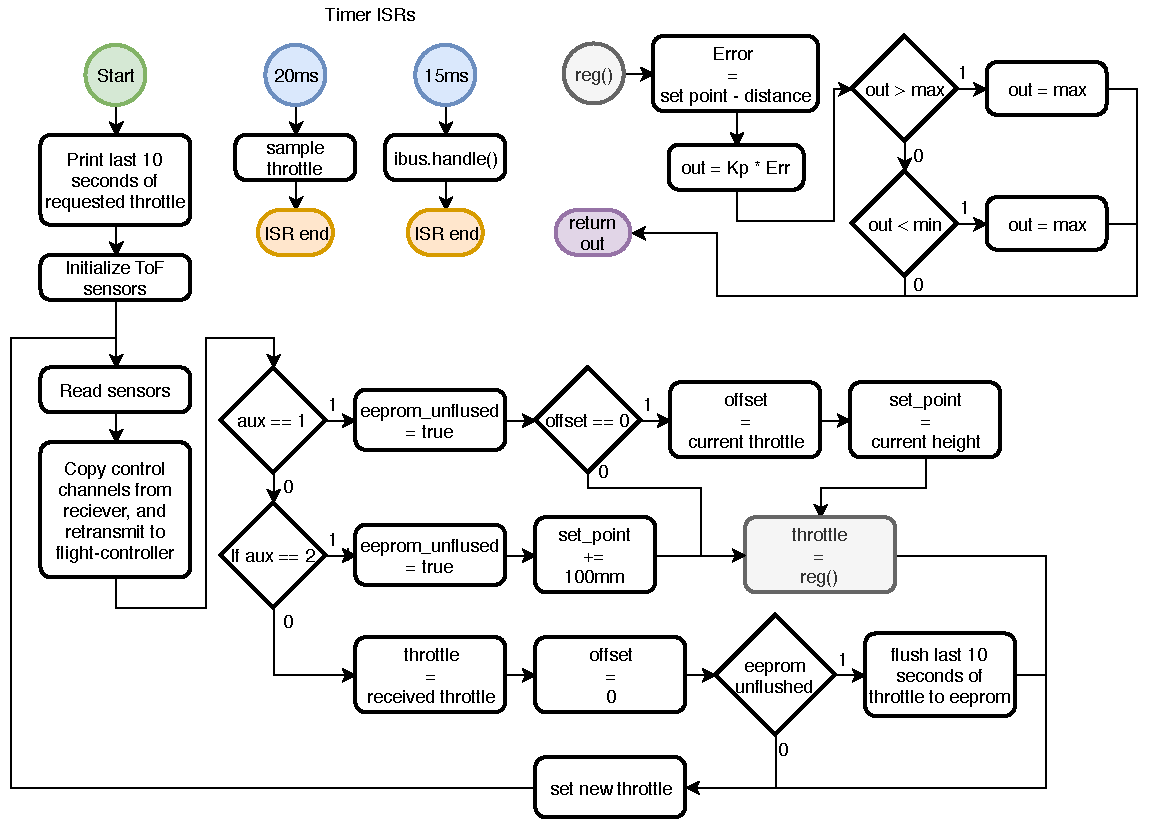
\includegraphics[width=1\textwidth]{figures/ch_design/controller/EIT5-code.pdf}
    \caption{Flowchart of the embedded system.}
    \label{fig:code_flowchart}
\end{figure}

The flow-chart can be broken into 4 major blocks. First is the power-on initialization, which is the first 2 blocks following the green "start". The second logical block would be the two different Interrupt Service Routines or ISRs starting with a blue circle, and ending on an orange bar. Third would be the regulator function, starting with a gray circle, and returning with a purple bar, and the fourth block would be the main program loop, consisting of the entire bottom part of the flow-chart.

\subsection*{Initialization}
This code runs once on start up, and waits 5 seconds for a serial connection to be established on it's USB port. If a serial instance is started, it prints out 1000 samples of the last 20 seconds of regulated throttle stored in EEPROM as comma separated values.
Then it sets up regularly timed ISRs, one to handle the iBUS communication every 15 ms, and one to sample the currently set throttle every 20 ms.
The Teensy 3.2 supports prioritized interrupts, and as such, the communication handling has been given a higher priority, as without it, the drone could shut off mid-flight.

\subsection*{ISRs}
The two ISRs are quite different, both in size and execution time.
The smallest is the \textit{"sample throttle"} ISR, which samples the currently set throttle value to a FIFO-buffer of 1000 samples. This is done both to limit EEPROM writes, and to keep it quick.\\

The second ISR runs the \textbf{\textit{handle()}} function of the iBUS object. This is a larger function that, best case, reads no bytes, and transmits 31 bytes. 
Worst case the function spends 2 ms reading incoming serial bytes, then sending a 31 byte iBUS packet.
Most of the time, the function will have 3.75 iBUS-packets waiting in its RX buffer, and have to send 1. If we round this up to 5 31 byte iBUS-packets it has to handle in total and assume that covers overhead, then at 115200 baud, this function will at most, take $5 \cdot 31 \cdot \frac{1E6}{115200} = 1345.5$  $[\mu{}s]$ 
This is fine for an ISR run on the Teensy 3.2

\subsection*{Regulator}
For this project, as discussed in chapter \ref{ch:model_drone}, we've decided to use a proportional regulator. This is implemented in this function, where first the current error is calculated, then this error is multiplied with the gain Kp, and this output value is then constrained to be within two minimum and maximum values before being returned. 

\subsection*{Loop}
This is the constantly looping part of the code, and this consciously reads the sensors, and transparently passes the incoming iBUS packets to the flight-controller on the drone. After that, it checks if the aux channel used for initiating regulation is in one of three states.\\

\textbf{0:}
If it's in state 0, the throttle is read from the incoming iBUS packets, and passed to the drone, allowing for complete manual flight of the drone, additionally this state resets if throttle-offset the drone uses when regulating, and if the drone has been regulating, it flushes the last 20 seconds of throttle values to EEPROM.\\

\textbf{1:}
If it's in state 1, and the offset hasn't been set yet, the drone will save the current throttle as the offset required to hover, and will then set the set-point for regulation, to the current height.
This allows the drone operator to fly the drone to a height where it hovers, before enabling regulation. 
It will then run the regulator, assigning the output to the throttle channel

\textbf{2:}
If it's in state 2, it will run the regulator with a +100mm set-point, compared to state 1.

\subsection*{Usage of the system}
With the code described, it becomes clear how the system is used to control the drone.

First, the drone operator flies it to a hover manually, and then enables regulation. This will set the set point to the current altitude, and set the gravity offset to the current thrust. Secondly, the operator can enable the second set point, which is +100mm.
